\documentclass[11pt,letter]{article}
\usepackage{amsmath, amsthm, amssymb}
\usepackage{eucal, mathrsfs, yfonts}
\usepackage{amsfonts}
\usepackage{amssymb}
\usepackage{amsmath}
\usepackage{amsthm}
\usepackage{verbatim}
\usepackage{fancyhdr}
\usepackage{geometry}
\usepackage{setspace}
\usepackage{Tabbing}
\usepackage{lastpage}
\usepackage{extramarks}
\usepackage{chngpage}
\usepackage{soul,color}
\usepackage{graphicx,float,wrapfig}
\usepackage[urlcolor=blue]{hyperref}
\hypersetup{colorlinks=true}

\graphicspath{{./Pictures/}}

%code preamble
\usepackage{color}
\usepackage{xcolor}
\usepackage{listings}

\usepackage{caption}
\DeclareCaptionFont{white}{\color{white}}
\DeclareCaptionFormat{listing}{\colorbox{gray}{\parbox{\textwidth}{#1#2#3}}}
\captionsetup[lstlisting]{format=listing,labelfont=white,textfont=white}

\lstset{language=C++,
               basicstyle=\ttfamily\small,
               keywordstyle=\color{blue}\ttfamily,
               otherkeywords={WIDTH},
               keywords=[2]{__shared__},
               keywordstyle=[2]\color{orange}\ttfamily,
               stringstyle=\color{green}\ttfamily,
               commentstyle=\color{red}\ttfamily,
               breaklines=true,
}
%end code preamble

\topmargin=-0.45in      %
\evensidemargin=0in     %
\oddsidemargin=0in      %
\textwidth=6.5in        %
\textheight=9.0in       %
\headsep=0.25in         %


\newcommand{\HRule}{\rule{\linewidth}{0.5mm}}

\pagestyle{fancy}

%-------------------------------------------------------------------------
%TITLE AND HEADERS
%-------------------------------------------------------------------------

\lhead{Asssignment 5}
\chead{UCID: 22365174}
\rhead{Arturo Pacifico Griffini}

\title{Assignment 5}
\author{Arturo Pacifico Griffini\\
  UCID: 22365174}
\date{}

\begin{document}
%\maketitle
%\input{./title.tex}

\pagebreak

%-------------------------------------------------------------------------
%PROBLEMS
%-------------------------------------------------------------------------


\section{Reduce}

\begin{lstlisting}[label=some-code,caption=reduce.cpp]
#include <cstring>
#include <cstdio>
#include <cstdlib>
#include <string>
#include <cmath>
#include <unistd.h>

#include "clhelp.h"

#define GROUP_SIZE 256
#define WORK_GROUPS 256

int main(int argc, char *argv[])
{
  std::string reduce_kernel_str;

  std::string reduce_name_str =
    std::string("reduce");
  std::string reduce_kernel_file =
    std::string("reduce.cl");

  cl_vars_t cv;
  cl_kernel reduce;

  readFile(reduce_kernel_file,
	   reduce_kernel_str);

  initialize_ocl(cv);

  compile_ocl_program(reduce, cv, reduce_kernel_str.c_str(),
		      reduce_name_str.c_str());

  int *h_A, *h_Y;
  cl_mem g_Out, g_In;
  int n = (1<<24);

  int c;
  /* how long do you want your arrays? */
  while((c = getopt(argc, argv, "n:"))!=-1)
    {
      switch(c)
	{
	case 'n':
	  n = atoi(optarg);
	  break;
	}
    }
  if(n==0)
    return 0;

  h_A = new int[n];
  h_Y = new int[n];

  for(int i = 0; i < n; i++)
    {
      h_A[i] = 1;
      h_Y[i] = 0;
    }

  cl_int err = CL_SUCCESS;
  g_Out = clCreateBuffer(cv.context,CL_MEM_READ_WRITE,
			 sizeof(int)*n,NULL,&err);
  CHK_ERR(err);
  g_In = clCreateBuffer(cv.context,CL_MEM_READ_WRITE,
			sizeof(int)*n,NULL,&err);
  CHK_ERR(err);

  //copy data from host CPU to GPU
  err = clEnqueueWriteBuffer(cv.commands, g_Out, true, 0, sizeof(int)*n,
			     h_Y, 0, NULL, NULL);
  CHK_ERR(err);


  err = clEnqueueWriteBuffer(cv.commands, g_In, true, 0, sizeof(int)*n,
			     h_A, 0, NULL, NULL);
  CHK_ERR(err);



  size_t local_work_size[1] = {GROUP_SIZE};
  size_t global_work_size[1] = {WORK_GROUPS * GROUP_SIZE};

  double t0 = timestamp();
  /* CS194 : Implement a
   * reduction here */
  err = clSetKernelArg(reduce, 0, sizeof(cl_mem), &g_In);
  CHK_ERR(err);
  err = clSetKernelArg(reduce, 1, sizeof(cl_mem), &g_Out);
  CHK_ERR(err);
  err = clSetKernelArg(reduce, 2, sizeof(float) * WORK_GROUPS, NULL);
  CHK_ERR(err);
  err = clSetKernelArg(reduce, 3, sizeof(int), &n);
  CHK_ERR(err);
  err = clEnqueueNDRangeKernel(cv.commands,
			       reduce,
			       1,//work_dim,
			       NULL, //global_work_offset
			       global_work_size, //global_work_size
			       local_work_size, //local_work_size
			       0, //num_events_in_wait_list
			       NULL, //event_wait_list
			       NULL //
			       );
  CHK_ERR(err);

  t0 = timestamp()-t0;

  //read result of GPU on host CPU
  err = clEnqueueReadBuffer(cv.commands, g_Out, true, 0, sizeof(int)*n,
			    h_Y, 0, NULL, NULL);
  CHK_ERR(err);

  //complete reduction serially
  for (int i = 1; i < WORK_GROUPS; ++i) {
    h_Y[0] += h_Y[i];
  }

  int sum=0.0f;
  for(int i = 0; i < n; i++)
    {
      sum += h_A[i];
    }

  if(sum!=h_Y[0])
    {
      printf("WRONG: CPU sum = %d, GPU sum = %d\n", sum, h_Y[0]);
      printf("WRONG: difference = %d\n", sum-h_Y[0]);
    }
  else
    {
      printf("CORRECT: %d,%g\n",n,t0);
    }

  uninitialize_ocl(cv);

  delete [] h_A;
  delete [] h_Y;

  clReleaseMemObject(g_Out);
  clReleaseMemObject(g_In);

  return 0;
}
\end{lstlisting}

\begin{lstlisting}[label=some-code,caption=reduce.cl]
__kernel void reduce(__global int *in, __global int *out,
		     __local int *buf, int n)
{
  size_t local_id = get_local_id(0);
  size_t group_id = get_group_id(0);
  size_t global_id = get_global_id(0);
  //semi sequential stage of the algorithm
  float accumulator = 0;
  int global_index = global_id;
  while (global_index < n) {
    accumulator += in[global_index];
    global_index += get_global_size(0);
  }
  buf[local_id] = accumulator;
  barrier(CLK_LOCAL_MEM_FENCE);
  //done with sequential stage

  //parallel stage
  for (int offset = get_local_size(0) / 2;
       offset > 0;
       offset = offset / 2) {
    if (local_id < offset) {
      buf[local_id] += buf[local_id + offset];
    }
    barrier(CLK_LOCAL_MEM_FENCE);
  }
  //done with parallel stage of algorithm

  //store in out
  if (local_id == 0) {
    out[group_id] = buf[0];
  }
}
\end{lstlisting}

\section{Scan}
The scan is performed recursively. Every work group performs a parallel implementation of scan on the chunk of data they get assigned and store the result in out. The scan.cl kernel also stores the greatest value of every chunk indexed according to the work group id in another buffer. Finally the update scan adds the values in the second buffer to the adjacent groups on the right completing the scan. 
\begin{lstlisting}[label=some-code,caption=scan.cl]
__kernel void update(__global int *in,
		     __global int *block,
		     int n)
{
  size_t idx = get_global_id(0);
  size_t tid = get_local_id(0);
  size_t dim = get_local_size(0);
  size_t gid = get_group_id(0);

  if(idx < n && gid > 0)
    {
      in[idx] = in[idx] + block[gid-1];
    }
}

__kernel void scan(__global int *in,
		   __global int *out,
		   __global int *bout,
		   __local int *buf,
		   int n)
{
  size_t idx = get_global_id(0);
  size_t tid = get_local_id(0);
  size_t dim = get_local_size(0);
  size_t gid = get_group_id(0);

  /* CS194: Write this kernel! */
  __local int buffer2[128];
  buf[tid] = in[idx];
  barrier(CLK_LOCAL_MEM_FENCE);
  for (int offset = 1; offset < dim; offset *= 2) {
    if (tid >= offset) {
       buffer2[tid - offset] = buf[tid - offset];
    }
    barrier(CLK_LOCAL_MEM_FENCE);
    if (tid >= offset) {
      buf[tid] = buffer2[tid - offset] + buf[tid];
    }
    barrier(CLK_LOCAL_MEM_FENCE);
  }
  out[idx] = buf[tid];
  if (tid == dim - 1) {
    bout[gid] = buf[tid];
  }
}
\end{lstlisting}

%\begin{figure}[h]
%\centering
%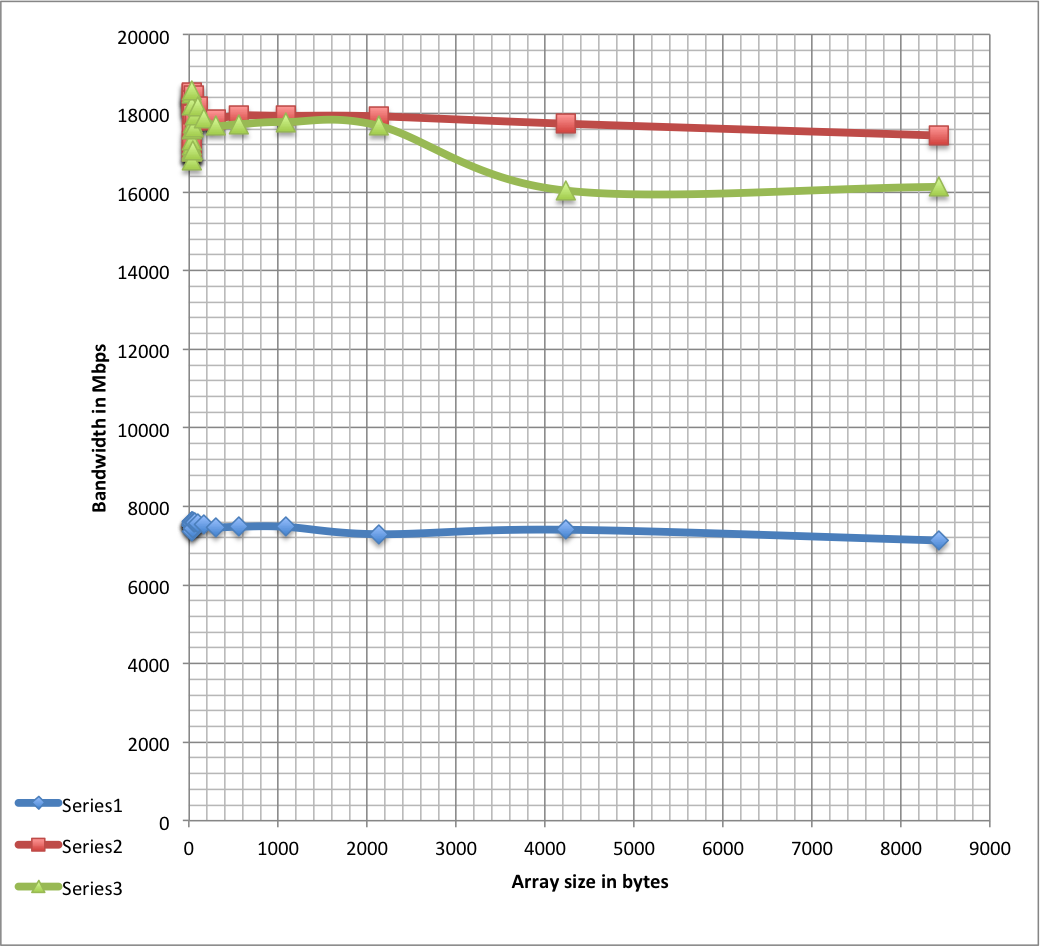
\includegraphics[width=0.8\textwidth]{graph_mem.png}
%\caption{series 1: inefficient routine; series 2: simd\_memcpy; series 3: simd\_memcpy\_cache}
%\label{fig:awesome_image}
%\end{figure}



\end{document}








% \begin{lstlisting}[label=some-code,caption=Some Code]
% public void here() {
% goes().the().code()
% }
% \end{lstlisting}








